\chapter{高阶拓扑绝缘体}
Edge mode 的波函数不只是会堆积在边界,还会堆积在平面系统的四个角上。前面已经展示了如何使用Berry connection来计算霍尔电导。实际上Berry connection也可以被用来计算电偶极矩
\begin{equation}
P_{1}=-\frac{e}{2 \pi} \int_{B Z} \operatorname{Tr}[A]
\end{equation}
这里的$A$是Berry connection。

电偶极矩的产生物理图像可以用上一节的edge mode来解释。当系统存在edge mode时,边界会有局域化的波函数,也就会有电荷堆积在边界。系统两个对立的边界电荷堆积量不同则形成了电偶极矩。这个电偶极矩的概念已经被推广到了三维材料,但是到了2017年才被Wladmir等研究人员在理论上推广到更高阶的电多极矩,而这正是波函数局域在系统角的体现\cite{hoti}。他们使用的其中一个模型如图\ref{hotimodel}所示
 \begin {figure}[tbp]
\centering 
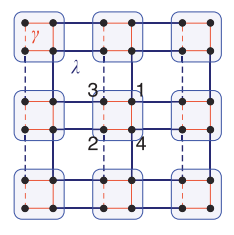
\includegraphics[width=6cm]{./images/HOTIModel.png} 
\caption{具有量子化电四极矩的紧束缚模型。$\Gamma$ 和$\lambda$表示格点间相互作用强度。虚
线表示负的强度。非平凡的拓扑相会在$|\gamma / \lambda| < 1$ 时出现}
\label{hotimodel}
\end {figure} 

若这个体系在x和y方向上都是周期边界,可以直接写出其哈密顿量
\begin{equation}
h^{q}(k, \delta)=\left[\gamma+\lambda \cos \left(k_{x}\right)\right] \Gamma_{4}+\lambda \sin \left(k_{x}\right) \Gamma_{3}+\left[\gamma+\lambda \cos \left(k_{y}\right)\right] \Gamma_{2}+\lambda \sin \left(k_{y}\right) \Gamma_{1}+\delta \Gamma_{0},
\end{equation}
其中$\Gamma_0 = \tau_3 \sigma_0, \Gamma_k = - \tau_2 \sigma_k, \Gamma_4 = \tau_0
\sigma_0$, k可取为1或2. $\tau$ 和 $\sigma$ 表示原胞的泡利矩阵。这个哈密顿量是一
个$4 \times 4$的矩阵,因此会有四个能带。为了观察到edge mode,我们把系统x,y方向
都改为开边界,并在实空间中数值解哈密顿量矩阵。那么它的本征值随参数$\gamma/\lambda$的变化如图\ref{hotiband}.a所示。
 \begin {figure}[tbp]
\centering 
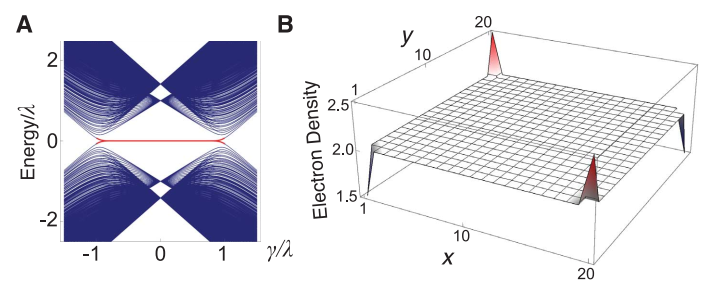
\includegraphics[width=14cm]{./images/HOTIBand.png} 
\caption{(a)以$\gamma / \lambda$为参数的系统的能谱图,红线表示四重简并的,在角处
局域化的态。(b)系统的电子密度。在每一个角上做积分得到的总电荷是正负$e/ 2$}
\label{hotiband}
\end {figure} 

这个图被分为上下对称的8个瓣。有些瓣之间有重叠,但这并不代表着能带会交叠。对于一
个特定的$\gamma/ \lambda$,系统有$4 \times N \times N$个本征值。4是由于原胞内的4
个原子。$N \times N$则来源于x和y方向上的N个原胞。如果体系在y上是周期边界的话,可
以把这$4 \times N \times N$个本征值按$k_y$为x轴来排列,得到对于特定$\gamma/ \lambda $的能带图。不同能带之间应该是没有交叠的(除了edge mode)。
当$\gamma/ \lambda > 1$时,从图\ref{hotiband}.a可以看出系统有明显的能隙,无edge mode,因此是拓扑
平凡体系。但是当$\gamma/ \lambda < 1$,图中间有一条红线穿过,表示在能隙中存在
edge mode,是拓扑非平凡的。拓扑非平凡表示体系在边界处有局域化波函数,但是在这个
特殊的模型里,波函数实际上是局域在体系的4个角上,因此电荷也是堆积在4个角上(图\ref{hotiband})。堆积
量为分数电荷量:$e / 2$ 或$-e/2$,所以这个体系会有电四极矩。